\documentclass[aps,prd,onecolumn,fleqn,superscriptaddress,groupedaddress,nofootinbib,preprintnumbers,nobalancelastpage]{revtex4}
\pdfoutput=1
\usepackage{amsmath,amssymb,pstricks,graphicx}

\begin{document}
\preprint{SLAC-PUB-?????, MCNET-18-??}
\title{Precision comparisons of predictions for Z/H + jet
and di-jet production at the LHC as a function of jet size}

%\author{Johannes Bellm}
%\affiliation{Lund University}
%\author{Xuan Chen}
%\affiliation{University of Zurich}
%\author{James Currie}
%\affiliation{University of Zurich}
%\author{Aude Gehrmann-De Ridder}
%\affiliation{ETH Zurich}
%\author{Thomas Gehrmann}
%\affiliation{University of Zurich}
%\author{Nigel Glover}
%\affiliation{IPPP Durham}
%\author{Alexander Huss}
%\affiliation{CERN}
%\author{Joao Pires}
%\affiliation{Instituto Superior Tecnico}
%\author{Stefan H{\"o}che}
%\affiliation{SLAC National Accelerator Laboratory}
%\author{Joey Huston}
%\affiliation{Michigan State University}
%\author{Silvan Kuttimalai}
%\affiliation{SLAC National Accelerator Laboratory}
%\author{Simon Pl{\"a}tzer}
%\affiliation{University of Vienna}
%\author{Emanuele Re}
%\affiliation{LAPTH Annecy-le-Vieux}
  
\begin{abstract}
  We perform a phenomenological study of
  $Z$ plus jet, Higgs plus jet and di-jet production
  at the Large Hadron Collider. We investigate in particular
  the dependence of the leading jet cross section on the
  jet radius as a function of the jet transverse momentum. 
  Theoretical predictions are obtained using perturbative QCD
  calculations at the next-to and next-to-next-to-leading order.
  They are compared to results obtained from matching 
  next-to-leading order calculations to parton showers.
\end{abstract}

\maketitle
\section{Introduction}
During Les Houches 2015~\cite{Badger:2016bpw}, a detailed 
comparison of fixed order (at NLO and NNLO) and matrix element plus parton shower (MEPS) predictions for differential Higgs
boson (+jet) production was carried out. The goal was multi-fold: using identical
starting configurations, to check the consistency of the MEPS
predictions among themselves, and to demonstrate that that the MEPS
predictions revert to their underlying fixed order predictions in
non-Sudakov kinematic regions. 
These comparisons largely showed good agreement among the ME+PS predictions and 
 that the ME+PS predictions agreed reasonably well with their fixed order counterparts. 

We have continued these studies in Les Houches 2017, but now looking in finer detail at 
the level of agreement. In particular, the perturbative jet shape is not as
well-defined at fixed order as with the NLO matrix element plus parton shower
predictions that are available. This may have a quantitative impact on the cross
section predictions, especially for small jet sizes.   

The study is designed to use Higgs+jet, Z+jet and inclusive jet production,
taking advantage of the NNLO calculations available for all three processes.
% It
%will be interesting to examine whether the good agreement between fixed order
%and ME+PS predictions observed for H+jet in the 2015 study holds for Z+jet and
%inclusive jet. 
The latter two processes are important for global PDF fits, where
only fixed order predictions (along with the relevant non-perturbative
corrections) have been used. 
Due to time constraints, only the Higgs+jet process will be considered in detail
in these proceedings. The other two processes, along with Higgs+jet,  will be
included in a more comprehensive study in a future publication. 

As a  further test of the impact of parton showers versus fixed order, the jet
size was varied over the values 0.3,0.4,0.5,0.6,0.7,1.0, using the antikT jet
algorithm. Indirectly, this tests how well the one (two) extra gluon(s) at
NLO(NNLO) reproduce the perturbative aspects of the jet shapes, as embodied by
the parton shower. This is of particular interest as the Higgs boson + jets measurements that have been performed at the LHC in Run 2 have used a jet size of 0.4, which is 
slightly above the jet size region where small R effects may be important. Taking them into proper account would require resummation, as discussed in ~\cite{}. The MEPS predictions also basically provide this resummation, through the parton showers. The 
MEPS predictions at NLO can properly take these effects into account. However, the highest precision for $H+\ge1$ jet is from the NNLO predictions, and there is no MEPS formalism that works at this order.   As an additional motivation, there has been recent speculation that the quark jet shape is
not well-described at NLO. This study provides samples of both quark and gluon
jets to test this hypothesis.

  Predictions from MEPS programs were carried out
at the parton shower level (for easiest comparison to fixed order)~\footnote{In
the future publication, comparisons will also be made at hadron level, as a way
of comparing the non-perturbative corrections as a function of jet radius.  As a
reminder, the non-perturbative corrections used for fixed order predictions are
determined from a comparison of the parton shower predictions with and without
the non-perturbative effects, as a function of jet radius. This implicitly
requires the integrated jet shape determined by fixed order predictions to agree
with those determined by parton showers.}.

Since the NLO predictions are also easily generated, the variation of the jet
size also allows a determination of the K-factor (NNLO/NLO) as a function of R. 

To the degree to which it was possible, the initial conditions have been
constrained to be the same for all predictions. Each calculation used the
PDF4LHCNNLO\_30 PDFs~\cite{Butterworth:2015oua}, with its central value of
$\alpha_s(m_Z)$ of 0.118. As its name implies, this PDF has 30 error PDF sets
that completely determine the PDF uncertainty. The scale choices for all
predictions have been designed to be as similar as possible, 
providing a greater level of control than was available in the 2015 Les Houches
study. More detail will be
provided in the sub-sections dealing with each prediction. 
%As the PDF uncertainty is not under investigation in this study, only the
%central PDF has %been used. Each program uses its standard scale choice. For
%inclusive jets, the standard %scale choice has been $p_T^{jet}$, where this
%quantity refers to the transverse momentum %of each jet. Thus, if there are
%four jets in a NNLO event (for double-real corrections), %there will be four
%entries in the plot, with the matrix element for each evaluated at the %scale
%of this jet. This is the very definition of an inclusive cross section. 
%An alternative choice is to use as a scale the transverse momentum of the
%highest $p_T$ %jet in the event ($p_T^{jet max}$). The use of these two
%disparate scales creates a %sizable cross section difference at NNLO at low
%transverse momentum~\cite{Currie:%2017ctp}, outside of the nominal scale
%uncertainty around either scale. Previously, this %dependence has been examined
%for only a few jet sizes. This study allows a more detailed %investigation. 
A CMS Rivet routine from the 13 TeV  inclusive jet analysis~\cite{Khachatryan:2016wdh}, was
modified to add the different R values, as well as additional variables. This
Rivet routine was further modified for the Higgs boson + jet (and Z boson + jet)
studies. 

\begin{figure}
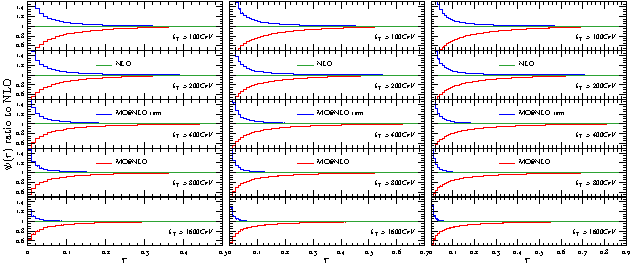
\includegraphics[width=\textwidth]{plots/shapes/hj/hjshapes-crop.pdf}\\
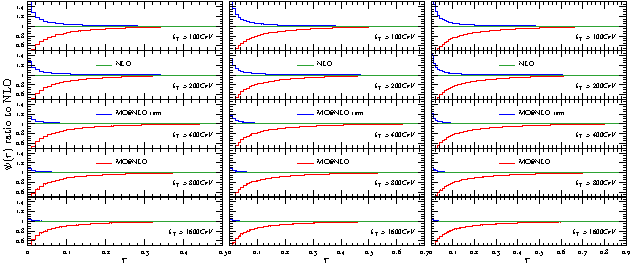
\includegraphics[width=\textwidth]{plots/shapes/zj/zjshapes-crop.pdf}
\caption{Jet shapes for Higgs and Z plus jets}
\end{figure}

\bibliography{journal.bib}

\end{document}
